%!TEX root = ../dissertation.tex
\chapter{Introduction}
\label{introduction}

In the last years the scientific community made significant progress
in the development of models for solving computer vision and natural
language processing tasks. The reasons behind those outstanding
advancements are manifold. In first place, the constant increase of
computational resources allows to exploit complex models which can
capture intricate behaviour. Secondly, the availability of new data
speed-up the learning process in terms of how we can benefit from
available information. However, the joint understanding of both
modalities is still an hard task, specially if we constraint the
problem within a deliberately simple and human-like environment.

Both visual and language modalities are required for solving
interesting, challenging and community worthwhile problems such us
visual question answering, image retrieval, robotic navigation and
visual grounding \todo{CITE PAPERS}. Among these, visual grounding
task is a foundamental building block and can be used to postulate
other tasks as a variation of the latter. A first abstract definition
for visual grounding could be:

\begin{quote}
    \textit{The task of locating the content of the image referenced
    by a given sentence.}
\end{quote}

Take for example the image in Fig.~\ref{fig:dog-playing-with-ball}
(top) and the phrase ``A collie plays with a white ball in a field of
green grass''. We can think to many solutions for the visual grounding
problem given that input. A first approach would be to grossly
localize the subject of the phrase in the image, thus, pratically
speaking, to draw a coarse box around the dog playing with the ball
(red box). Another solution instead would be to localize the ball, the
dog and the ground distinctly (yellow, red and blue boxes),
identifying precise regions of the image and draw precise boxes among
interesed objects. Both two solutions are legal and belong to the
visual grounding field. The former is known as referring expression
grounding (REG) while the latter as phrase grounding (PG). The main
difference between the two is the grain used to solve the problem, and
this has significant impacts on how we can approach the problem and
the relevance for other tasks.

\begin{figure}
    \centering
    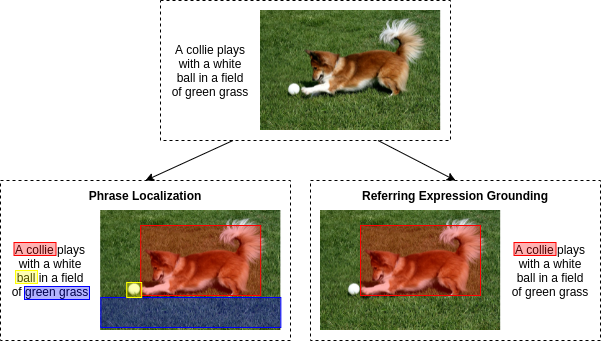
\includegraphics[width=0.9\textwidth]{figures/dog-playing-with-ball.png}
    \caption[Short figure name.]{This is a figure that floats inline and here is its caption. \todo{complete description and add two images, one for reg and the other for phrase grounding}
    \label{fig:dog-playing-with-ball}}
\end{figure}

With the availability of large datasets \todo{CITE DATASET PAPERS},
many different solution for the visual grounding task has been
proposed in literature, but most of them relies on expensive
annotations. We argue that this technique cannot scale and is becoming
a critical bottlenck: it is hard and expensive to collect grounding
information while very simple to collect images with their
descriptions. Also, the way humans learn phrase localization is by
assembling prior kwnowledge instead of memorize a mapping between
textual and image examples.

This encourages us to investigate the visual grounding task under the
weakly supervised setting. In weakly supervised scenario, the
available ground truth is a shallow information which links a
description with its own image and vice-versa. On the countraty, the
fully supervised setting provide also the information between noun
phrases and objects in image, while in unsupervised settings no ground
truth is available.

In this work, we propose a model for exploiting semantic information
convoyed by class labels on bounding box. We assert that, given a
phrase, the image should contain an object detected by an object
detector whose bounding box class label is similar to the head of
given phrase. \todo{rivedere la forma}
